\section{\label{sec:level1}Systematic Uncertainties}
 Systematic errors are caused the controls of the experiment, such as flux, simulation, density and length of the $\ell H_2$ target and also systematic errors are caused by various analytical tools used, such as the kinematic fitter.
 \subsection{Branching Ratio Systematic Uncertainty}
 The branching ratios for the two topologies used to measure the cross-section were obtained from \abbr{PDG}\label{abbr:pdg}~\cite{pdg} and are listed again in Table~\ref{tab:brspecs} with their associated errors. Uncorrelated quantities that are summed as,
 \begin{align}
 	f = \sum_{i = 1}^{M}a_iP_i  
 \end{align}
 have errors as
 \begin{align}
 	\sigma_f = \sqrt{\sum_{i = 1}^{M}\left(a_i\sigma_i\right)^2}.  
 \end{align}
 Therefore
 \begin{align}
 	\frac{\Gamma}{\Gamma_{tot}} &  = \frac{\Gamma_{\pi^{0}\rightarrow e^{+}e^{-}\gamma}}{\Gamma_{tot}} + \frac{\Gamma_{\pi^{0}\rightarrow \gamma \gamma \to e^{+}e^{-}\gamma}}{\Gamma_{tot}}  \\ & = \frac{\Gamma_{\pi^{0}\rightarrow e^{+}e^{-}\gamma}}{\Gamma_{tot}} + \frac{\Gamma_{\pi^{0}\rightarrow \gamma \gamma}P(\gamma \to  e^{+}e^{-})}{\Gamma_{tot}} \ ,
 \end{align}
 where $P(\gamma \to  e^{+}e^{-})$ is the probability of photon conversion into $e^+e^-$. To measure $P(\gamma \to  e^{+}e^{-})$, the acceptance for conversion ($P(\gamma \to  e^{+}e^{-})\cdot\eta_{e^+e^-}$) is divided by the acceptance for Dalitz ($\eta_{e^+e^-}$). Fig.~\ref{fig:convprob_all} shows that the conversion probability depends on incident photon energy. A maximum probability of 8\%  per-photon was measured, shown in Fig~\ref{fig:convprob_II} top left plot. 
 \begin{figure}[h!]\begin{center}
 		\subfloat[Probability of Photon Conversion vs. $\cos\theta$][]{ %Feynman diagram of \piz two photon decay
 			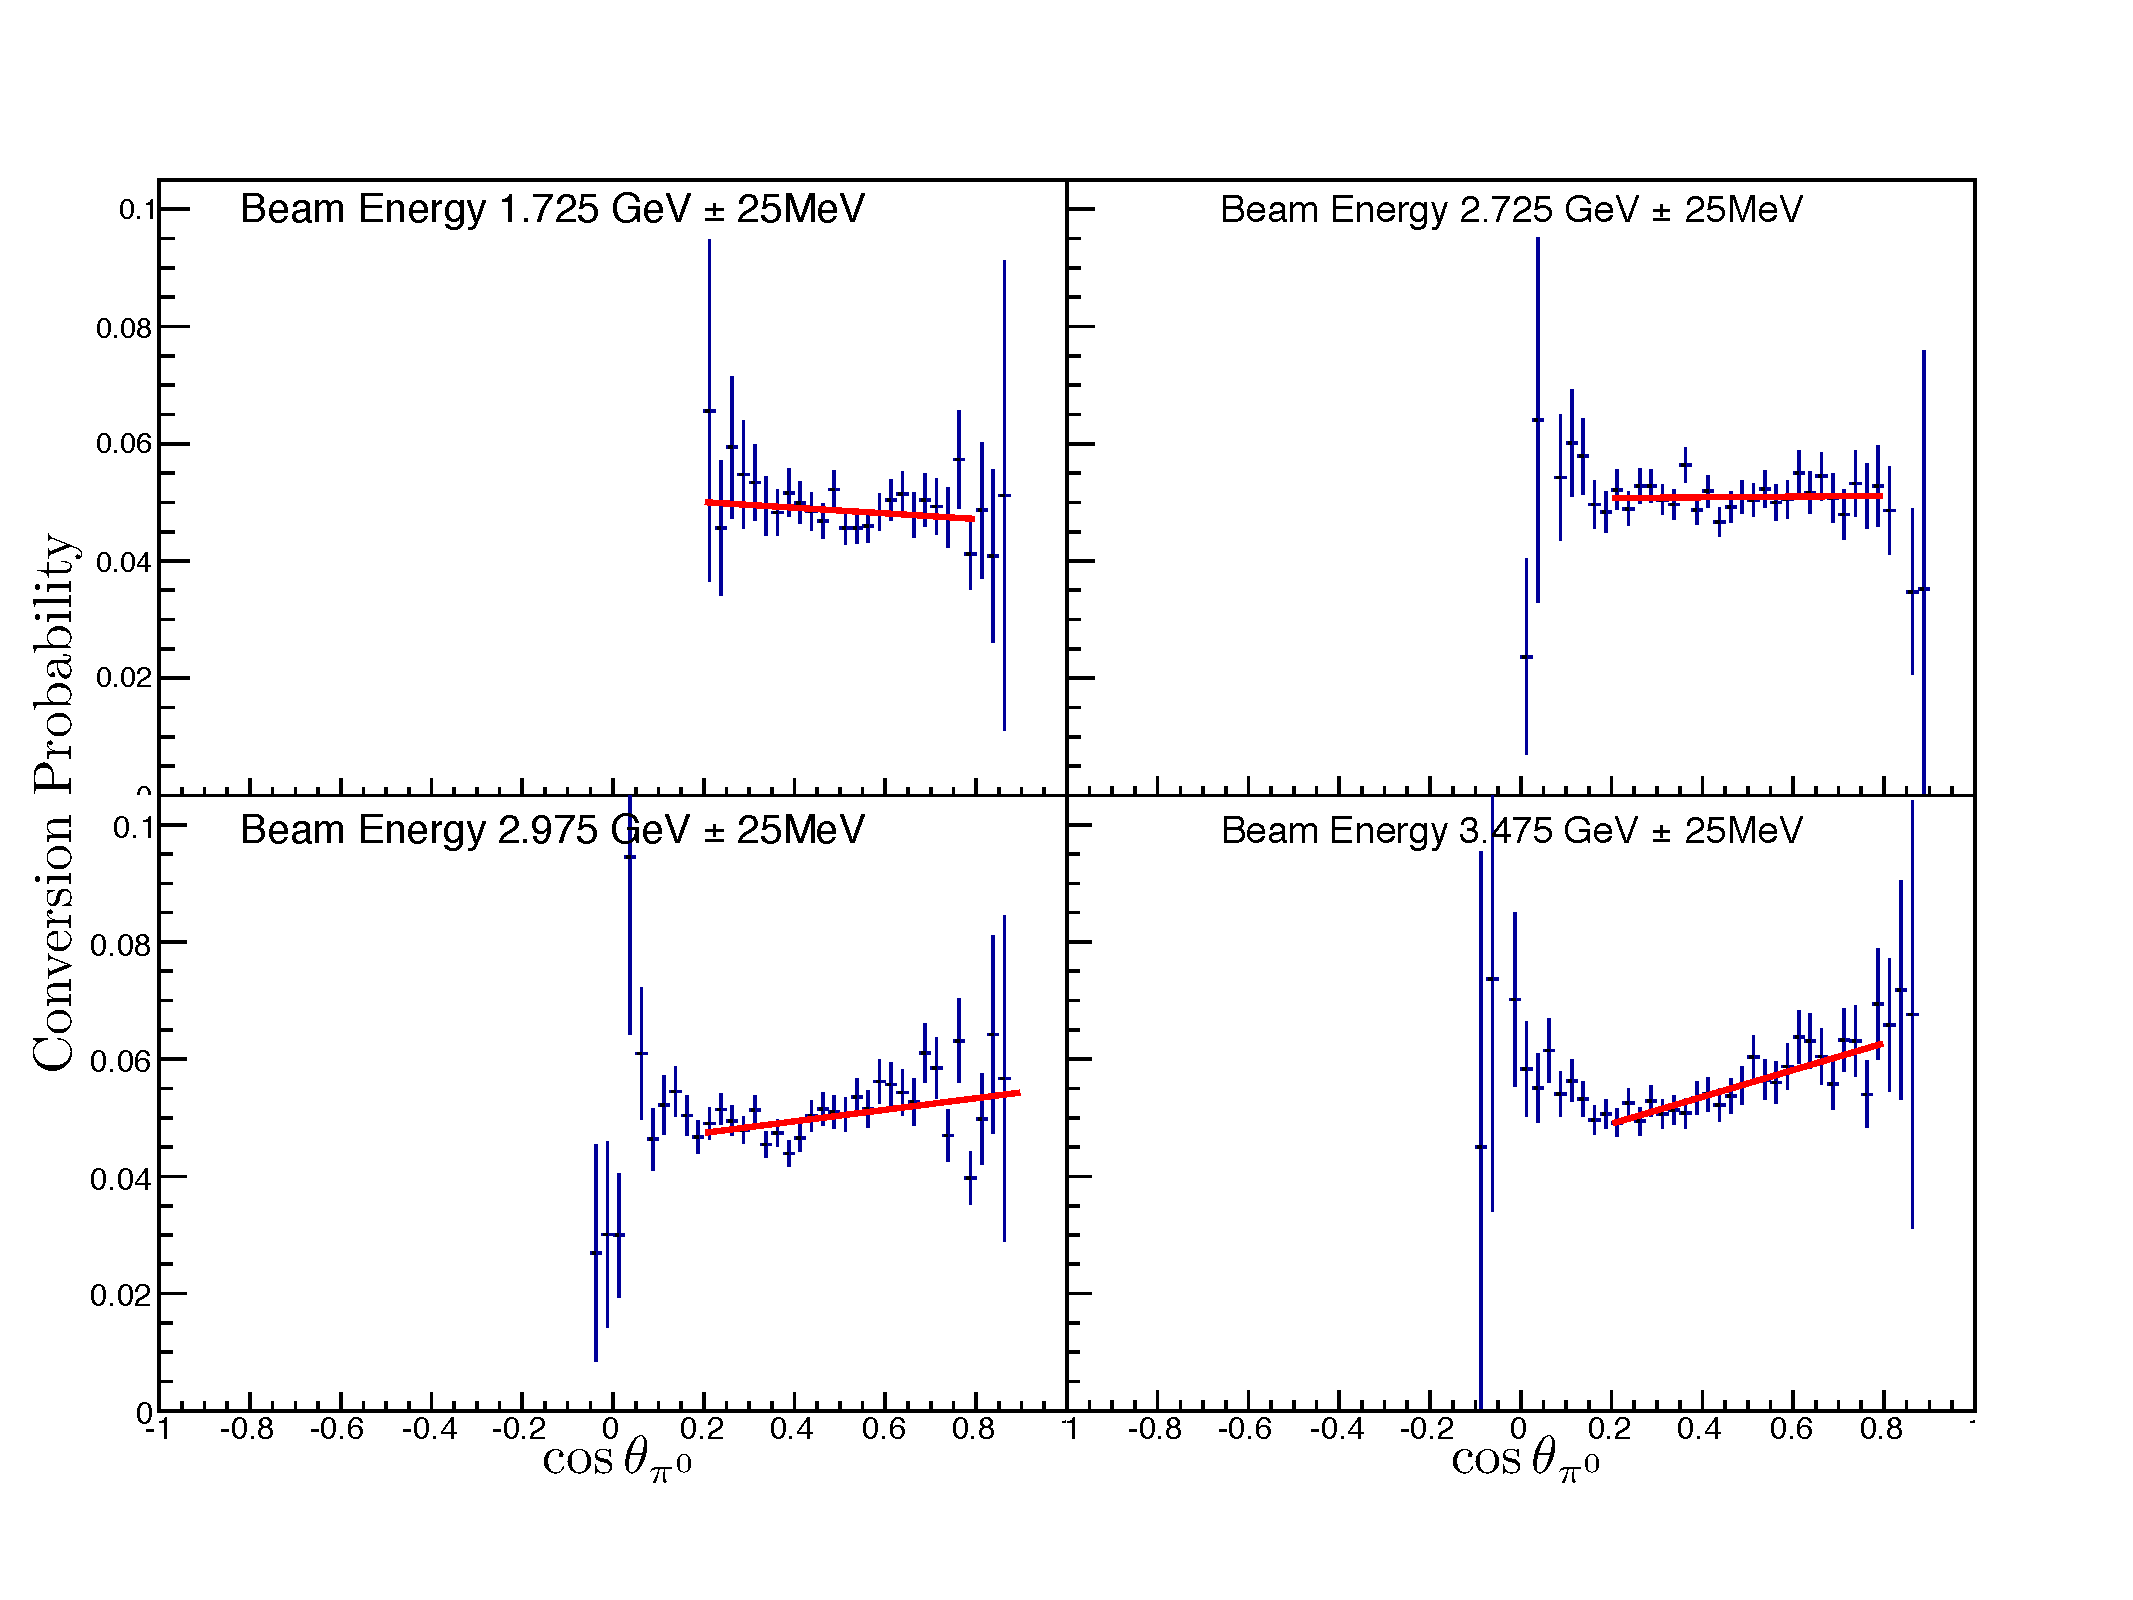
\includegraphics[width=\figwidth,height=\qfigheight]{\figures/SYSTEMATICS/Converion_Probability_fix.pdf}\label{fig:convprob_I}
 		}\\
 		\subfloat[Probability of Photon Conversion vs. $\cos\theta$][]{ %Feynman diagram of \piz Dalitz decay
 			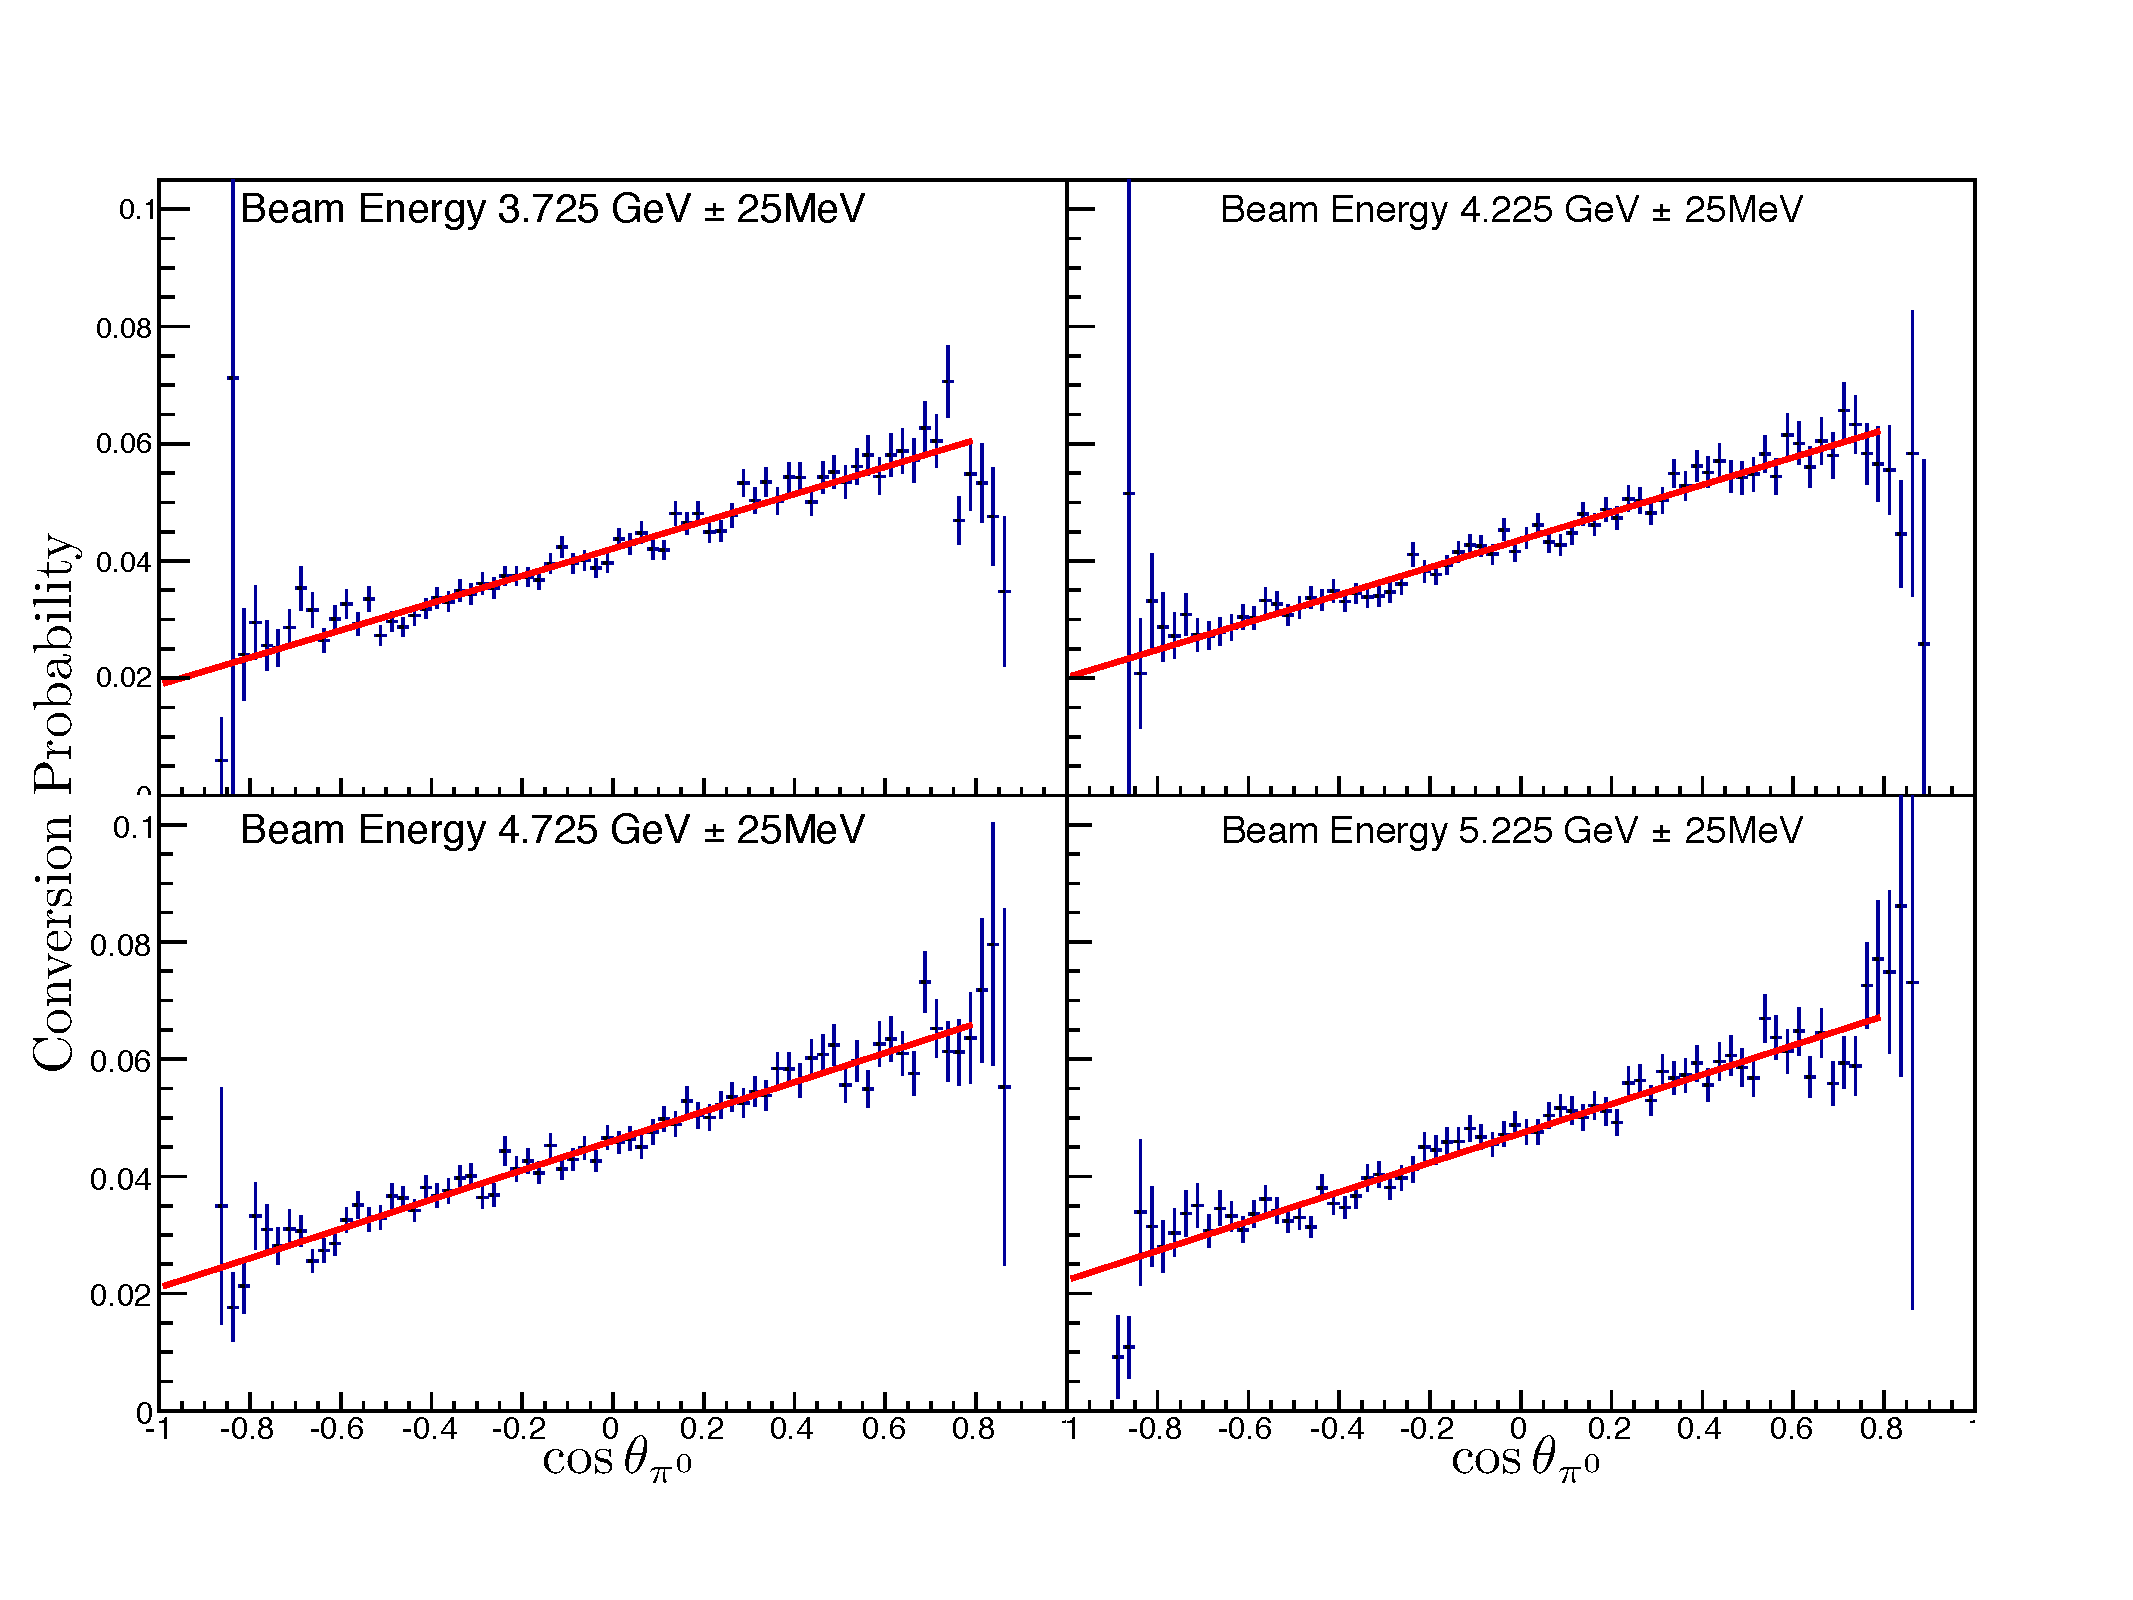
\includegraphics[width=\figwidth,height=\qfigheight]{\figures/SYSTEMATICS/Converion_Probability_II_fix.pdf}\label{fig:convprob_II}
 		}
 		\caption[Probability of Photon Conversion vs. $\cos\theta$ for various values of $E_\gamma$]{\label{fig:convprob_all}Probability of Photon Conversion vs. $\cos\theta$ for various values of $E_\gamma$. The maximum probability for this analysis was measured in the top left plot of b.}
 	\end{center}\end{figure}
 	Therefore
 	\begin{align}
 		\frac{\Gamma}{\Gamma_{tot}} = \frac{\Gamma_{\pi^{0}\rightarrow e^{+}e^{-}\gamma}}{\Gamma_{tot}} + \frac{\Gamma_{\pi^{0}\rightarrow \gamma \gamma}P(\gamma \to  e^{+}e^{-})}{\Gamma_{tot}} = 0.09 \ ,
 	\end{align}
 	and has error
 	\begin{align}
 		\sigma_f = \sqrt{\left(\frac{1}{\Gamma_{tot}}\right)^2(\sigma^2_{\pi^{0}\rightarrow e^{+}e^{-}\gamma} + \sigma^2_{\pi^{0}\rightarrow \gamma \gamma})  } = 0.0037.  
 	\end{align}
 	The energy and $\cos \theta$ dependence of the conversion is accounted for in the acceptance, which is $E_\gamma$ and $\cos \theta$ bin-dependent. 
 	\begin{table}[h!]
\begin{minipage}{\textwidth}
\begin{center}


\caption[Branching Ratios of \piz]{\label{tab:brspecs}Branching ratio and errors used in $\frac{d\sigma}{d\cos\theta^{\pi^0}_{C.M.} d\phi}$ measurements \vspace{0.75mm}}

\begin{tabular}{c|c|c}

\hline
Quantity & Value & Error \\
\hline
$\Gamma_{\pi^{0}\rightarrow \gamma \gamma }$& 0.98823 & 0.00034 \\
$\Gamma_{\pi^{0}\rightarrow e^{+}e^{-}\gamma}$ & 0.01174 & 0.00035 \\
$\frac{\Gamma}{\Gamma_{tot}}$ & 0.13 & 0.0037 \\
\hline \hline
\end{tabular}


\end{center}
\end{minipage}
\end{table}
\vspace{20pt}
 	
 	
 	\subsection{Cut Based Systematic Uncertainty}
 	The procedure to determine the systematic uncertainty of the cuts placed on the various kinematic fits was first to calculate an acceptance with a different cut, then to calculate a new total cross-section measurement applying the different cut to the data. The total cross-section was computed at various photon beam energies. Lets denote the original measured total cross-section as $\Xi_1$ and the new total cross-section determined by the new cut as $\Xi_n$, then the systematic error was calculated as.
 	
 	\begin{align}
 		\sigma_{cut} = \frac{\left| \Xi_1 - \Xi_n \right|}{\Xi_1}
 	\end{align}
 	
 	Some systematic uncertainty depended on the photon energy. All cut based systematics were performed individually, meaning when a cut was changed, the remaining cuts retained their original value, see Table~\ref{tab:cutsystematics} for the values of the cuts that were changed to calculate the systematic error.
 	%This new cross-section was then compared to the cross-section using the base cuts to determine if a dependence on $\cos\theta^{\pi^0}_{C.M.})$ was present. All systematics of the cut based did not show a $\cos\theta^{\pi^0}_{C.M.})$ dependency for specific beam energies.
 	\begin{table}[h!]
\begin{minipage}{\textwidth}
\begin{center}


\caption[Variance of Data Cut Systematics]{\label{tab:cutsystematics}Different Cuts to analyze systematics \vspace{0.75mm}}

\begin{tabular}{c|c|c|c}

\hline
Cut & Original & Adjusted & Uncertainty \\
\hline
2-C Fit Pull Probability  & 1\% & 10\% & $0.0219$\\
1-C Fit Pull Probability & 1\% & 10\% & $ 0.00216 + 0.01083E_{\gamma}$ \\
4-C Fit Pull Probability  & 1\% & 10\% & $0.00031$\\
Missing Energy Cut  & 75~MeV & 100~MeV & $0.02781$\\
\hline \hline
\end{tabular}


\end{center}
\end{minipage}
\end{table}
\vspace{20pt}
% 	
% 	\begin{figure}[h!]\begin{center}
% 			\includegraphics[width=1.2 \figwidth,height=\hfigheight]{\figures/analysis/All_Cut_Systematic.pdf}
% 			\caption[Plot showing the contribution of the data cut systematic error and the incoming beam dependence of the error]{\label{fig:sys_cut_error} Plot showing the contribution of the data cut systematic error and the incoming beam dependence of the error.}
% 		\end{center}\end{figure}
%
\subsection{Photon Flux Systematic Uncertainty}
 		The photon flux calculation should be consistent throughout the experiment. If the flux measurement is not consistent due to corrections made with the live-time, beam corrections or fractional difference in the reported current to the actual current during the photon flux normalization run then a systematic uncertainty would be produced. To study this effect we divided the g12 run period into four groups. Table~\ref{tab:flux_sys} lists the run groups used for this study.
 		\begin{table}[h!]
\begin{minipage}{\textwidth}
\begin{center}


\caption[Run Groups Used to Determine Photon Flux Systematic Error ]{\label{tab:flux_sys}List of run groups used to determine photon flux systematic error. \vspace{0.75mm}}

\begin{tabular}{c|c|c}

\hline
Run Group & Range & Total Runs \\
\hline
1 & 56605-56798 & 116 \\
2 & 56799-56980 & 116 \\
3 & 56992-57173 & 116 \\
4 & 57174-57317 & 115 \\
\hline \hline
\end{tabular}


\end{center}
\end{minipage}
\end{table}
\vspace{20pt}
% 		
 		The procedure to determine the systematic error, $\sigma$, of the flux is to calculate the accepted and flux corrected yield, $\Upsilon^c$, for each run group and compare $\Upsilon^c$ to the average accepted and flux corrected yield of all 4 run groups, $\mu^c$. After $\sigma$ is calculated, it was normalized to $N \mu^c$ as to represent the error as a percentage, which later is added in quadrature and  multiplied by the measured cross section to determine the appropriate error. 
 		\begin{align}
 			\sigma_{group} = \sqrt{\sum_{i=1}^{N = 4}\left(\Upsilon_i^c - \mu^c\right)},
 		\end{align}
 		where
 		\begin{align}
 			\mu^c = \frac{1}{N}\sum_{i=1}^{N=4}\Upsilon_i^c
 		\end{align}
 		\begin{align}
 			\sigma_{group}^{normalized} = \frac{\sigma_{group}}{N\mu^c}
 		\end{align}
 		
% 		\begin{figure}[h!]\begin{center}
% 				\includegraphics[width=1.2 \figwidth,height=\hfigheight]{\figures/analysis/Beam_Fluxsystematic_Error.pdf}
% 				\caption[Plot showing the contribution of the flux systematic error and the incoming beam dependence of the error]{\label{fig:sys_flux_error} Plot showing the contribution of the flux systematic error and the incoming beam dependence of the error.}
% 			\end{center}\end{figure}

 			
 			
 			
 			\subsection{Detector Efficiency Systematic Uncertainty}
 			Each sector in \abbr{CLAS} can be treated as an individual detector, with its own efficiency and resolution. A systematic uncertainty could arise if one or more of the sectors is not simulated properly. The procedure to determine the systematic error, $\sigma$, of the sector is to calculate the accepted corrected yield, $\Upsilon^c$, for each sector and compare $\Upsilon^c$ to the average accepted corrected yield of all 6 sectors, $\mu^c$. After $\sigma$ is calculated, it was normalized to $N \mu^c$ as to represent the error as a percentage, which later is multiplied by the measured cross section to determine the appropriate error. 
 			\begin{align}
 				\sigma_{sector} = \sqrt{\sum_{i=1}^{N = 6}\left(\Upsilon_i^c - \mu^c\right)},
 			\end{align}
 			where
 			\begin{align}
 				\mu^c = \frac{1}{N}\sum_{i=1}^{N=6}\Upsilon_i^c
 			\end{align}
 			\begin{align}
 				\sigma_{sector}^{normalized} = \frac{\sigma_{sector}}{N\mu^c}
 			\end{align}
 			This calculation was performed for various bins of incoming beam energy to determine the beam energy dependence.% (see Fig.~\ref{fig:sys_sec_error}).
 			
% 			\begin{figure}[h!]\begin{center}
% 					\includegraphics[width= \figwidth,height=0.75\hfigheight]{\figures/analysis/Beam_systematic_Error.pdf}
% 					\caption[The sector systematic uncertainty as a function of the incoming photon energy]{\label{fig:sys_sec_error}The sector systematic uncertainty as a function of the incoming photon energy.}
% 				\end{center}\end{figure}
 				%The sector systematic uncertainty is consistent with the extracted sector systematic uncertainty from the g11 data set~\cite{williams}(seeFig.~\ref{fig:sys_sec_error.compare}).
% 				\begin{figure}[h!]\begin{center}
% 						\includegraphics[width= \figwidth,height=0.75\hfigheight]{\figures/analysis/S_systematic_Error.pdf}
% 						\caption[Comparison of sector systematic uncertainty to g11 measurement]{\label{fig:sys_sec_error.compare}Comparison of sector systematic uncertainty to g11 measurement.}
% 					\end{center}\end{figure}

 					
 					\subsection{$z$-vertex Cut Systematic Uncertainty}
 					The systematic uncertainty of the $z$-vertex cut was analyzed by varying the initial vertex cut from $-110 \le z \le -70$ to $-109 \le z \le -71$ for both data and \abbr{MC}. Afterward the procedure for determining the systematic was identical to the method used to determine the ``Cut Based Systematic Uncertainty". The systematic uncertainty from varying the $z$ was 0.0041, shown in Fig.~\ref{fig:results.syserr}
 					
 					\subsection{Target Systematic Uncertainty}
 					Since the systematic on the density is 0.02\%,see Sec~\ref{sec:analysis.target_density}, the maximum systematic on the target is due to uncertainty in the length on the target which is 40~cm $\pm$ 0.2~cm. A total systematic on the target was assign to be 0.5\%. 
 					
 					\subsection{Total Systematic Uncertainty}
 					The total systematic uncertainty along with a list of the individual systematics is presented in this subsection. The calculation of the total systematic error is 
 					\begin{align}
 						\sigma^{sys}_{tot} = \sqrt{\sum_{i=1}^{M}\sigma_i^2}
 					\end{align}
 					\begin{table}[h!]
\begin{minipage}{\textwidth}
\begin{center}


\caption[Systematics]{\label{tab:systematics}Systematic errors used in $\frac{d\sigma}{d\cos\theta^{\pi^0}_{C.M.} d\phi}$ measurements \vspace{0.75mm}}

%\begin{tabular}{c|c}
\begin{tabular}{p{5cm} | p{7cm}}
\hline
Systematic & Error \\
\hline
Sector  & $ 0.0361 + 0.0065E_{\gamma}$ \\
Flux  & $ -0.00051 + 0.00491E_{\gamma}$ \\
Missing Energy Cut  & $0.02781$ \\
2-C Fit Pull Probability & $0.0219$ \\
1-C Fit Pull Probability  & $ 0.00216 + 0.01083E_{\gamma}$ \\
4-C Fit Pull Probability  & $0.00031$ \\ 
Target  & $0.005$ \\
Branching Ratio  & $0.0037$ \\
Fiducial Cut & $0.024$ \\
$z$-vertex Cut & $0.0041$ \\
Total & $\sqrt{0.0032 +0.00051E_{\gamma} +0.000184E_{\gamma}^2}$ \\
\hline \hline
\end{tabular}


\end{center}
\end{minipage}
\end{table}
\vspace{20pt}
% 					Figure~\ref{fig:results.syserr} is a pictorial version of Table~\ref{tab:systematics}.
% 					\begin{figure}[h!]\begin{center}
% 							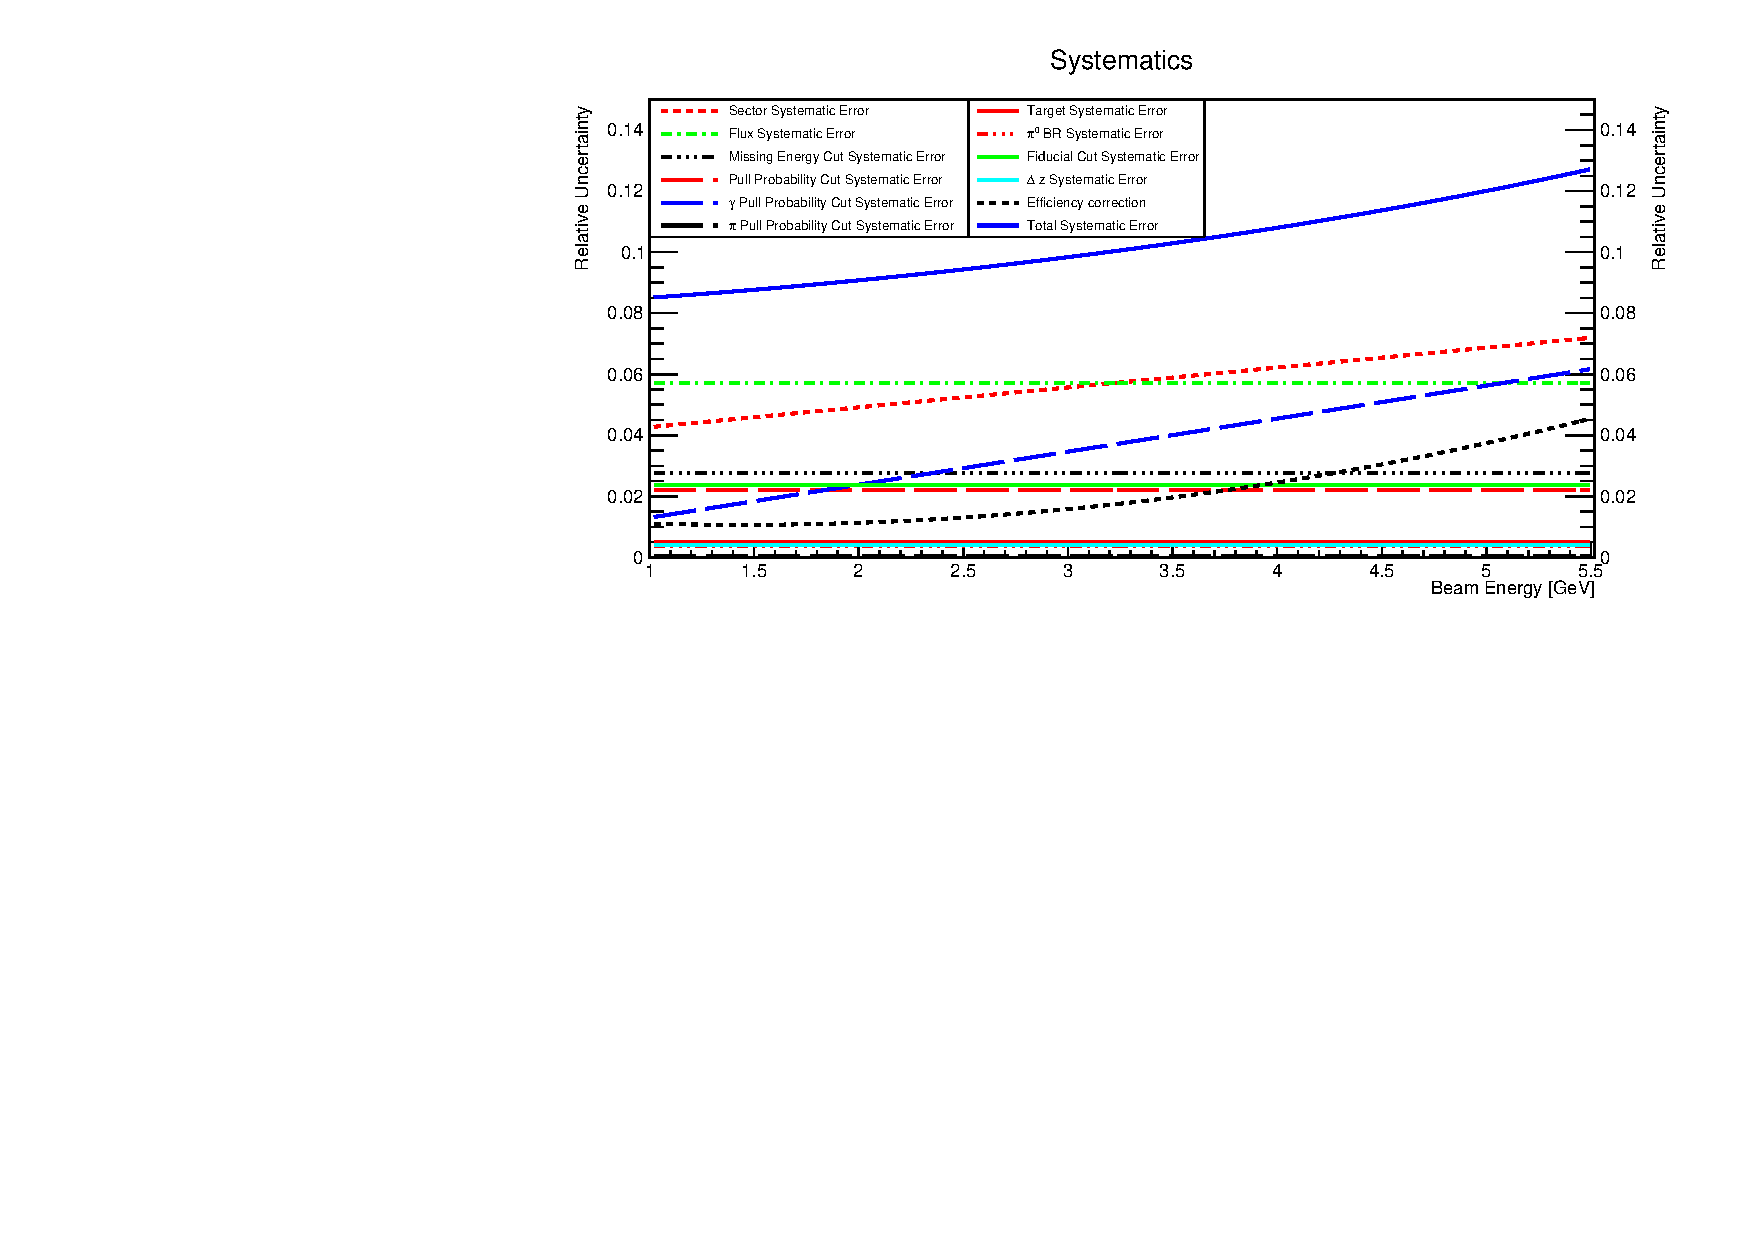
\includegraphics[width=1.1 \figwidth,height=\hfigheight]{\figures/SYSTEMATICS/All_Systematics.pdf}
% 							\caption[The contribution of all systematic uncertainties]{\label{fig:results.syserr}The contribution of all systematic uncertainties.}
% 						\end{center}\end{figure} 